\documentclass[conference]{IEEEtran}
\IEEEoverridecommandlockouts
% The preceding line is only needed to identify funding in the first footnote. If that is unneeded, please comment it out.
%\usepackage{cite} Incompatible with biblatex
\usepackage{amsmath,amssymb,amsfonts}
\usepackage{algorithmic}
\usepackage{graphicx}
\usepackage{textcomp} 
\usepackage{xcolor}
\usepackage[style=ieee]{biblatex}
\usepackage[toc,page]{appendix}
%\usepackage{hyperref}
\addbibresource{references.bib}
\def\BibTeX{{\rm B\kern-.05em{\sc i\kern-.025em b}\kern-.08em
    T\kern-.1667em\lower.7ex\hbox{E}\kern-.125emX}}

\begin{document}

\title{Which requirements favour which implementation? \\}

\maketitle

\begin{abstract}
This paper will dive in four different implementations of the Insertion Sort algorithm. The four implementations are FSMD (Finite State Machine with Data path), ASIP (Application-Specific Instruction-set Processor), a custom intellectual property (IP) block based on a high-level-synthesis and a pure implementation in C code. We describe the implementations first before comparing them in the aspects of design and implementation complexity, debugging experience, flexibility and reuseability, efficiency, concurrency, as well as production and implementation costs. The FSMD has its key benefits in the aspects of efficiency and concurrency. The ASIP is not as efficient and has less concurrency but enables flexibility and reuseability. The IP block has both some efficiency and concurrency and supports more flexibility and reuseability. The pure C code is the most cost-efficient solution with the lowest complexity. However, any advantages from a hardware implementation remain unutilized.
\end{abstract}

\section{Introduction}
In the scope of our project we implemented the sorting algorithm Insertion Sort in four different ways. Firstly, we implemented a FSMD followed by an ASIP. Then we moved on to a software solution with pure C code. This C code was then finally used to implement a custom IP. In a first part we present our experiences for developing the algorithm and illustrate the varrying complexity and difficulty of designing, implementation and debugging of the Insertion Sort. During the implementations we learned a lot about both the benefits and drawbacks for each solution.\\
In a second part, we are using our experience described in the first part as well as the theory we were thought in the lectures to compare the implementations from various different aspects. In general, these aspects should be taken into consideration when choosing an implementation form. For each aspect we highlight which implementation is best suited and we end with a conclusion that summarizes the comparison and also propose a situation in which each implementation should be used.

\section{Insertion Sort}
We decided to implement the Insertion Sort Algorithm for the project asignment. It is a well-known and simple sorting algorithm. The concept of Insertion Sort is akin to organizing playing cards in your hand: you divide the cards into two groups, the sorted and the unsorted. Then, you select a card from the unsorted group and insert it into the correct position in the sorted group~\cite{g4g}.\\
It is maily used for small or nearly sorted lists. For a nearly sorted list, the time complexity of Insertion Sort is a $O(n)$ which is the best case. The average and worst case have both a time complexity of $O(n^2)$. Other sorting algorithms such as Merge Sort and Quick Sort are more commonly used due to their lower average time complexities.\\
Insertion Sort is a in-place sorting algotithm which means that its space complexity is at $O(n)$. It needs the same amount of space as the input and only a fixed number of extra inputs.

\section{Implementations}
This section will focus on our four different implementations of the Insertion Sort algorithm. We implemented them in the order in which they are listed in the following sections. We wanted to start with a hardware implementation as we did not feel comfortable enough to start with the application-specific instruction set processor (ASIP) implementation. Therefore we decided to start with the finite state machine with data path (FSMD) implementation. This choice turned out to be helpful for both the ASIP and IP Block implementations. For the ASIP, we used the ASMD diagram from our FSMD implementation. Later during the creation of our custom intellectual property (IP) block, we started by using the same code which we used in our C-program. \\
The whole group worked together on each implementation, and we completed them one at a time. We made sure the current implementation was fully working before starting the next one. This lead to the work being non-ambigous and the entire group was on the same page during the whole project.

\subsection{FSMD}\label{section:fsmd}
Our implementation started with designing both the FSMD as well as the algorithm state machine with datapath (ASMD) diagram. As we learned in class, we created the FSMD diagram first since it helps for the ASMD to know which blocks can be used. There, we chose the parts that were needed such as a \texttt{RAM}, a Universal Asynchronous Receiver Transmitter (UART) for both receiving (\texttt{UART\_rx}) and transmission (\texttt{UART\_tx}) as well as comparators and registers. The \texttt{comparator} is doing what the name suggests - comparing two values. The output is a single bit reflecting the outcome of the comparisson. \\ 
Based on this we defined our data path in accordance to our components. In order to keep the implementation simple and close to the concept, we avoided sending any data to the control path. We exchanged only control signals. In the end we have nine input signals for our control path and twelve output signals that handle the dataflow in the data path.\\
After coming up with a FSMD we defined an ASMD. Here we devided our data flow into different states. Each state is one clock cycle long and therefore in- and output singals can only represent one value in each state. In total, there are ten states. State S0 resets the registers to start the sorting anew. S1 receives and saves the integers which are received via a serial connection to the RAM. The \textit{Enter} character will trigger the transition to start states S2 to S7. Here the received numbers are sorted iteratively. Unsorted numbers will be compared to the already sorted number sequence. This is done by starting from the high values and moving on the low values in the already sorted section. Any value which is higher then our next unsorted number will be swapped along the way. At the end the unsorted number is then inserted at the right place. This will be repeated until there are no unsorted numbers left and every number is at their right place. Again the transition to the next states is triggered by finding an \textit{Enter} character. In S8 and S9 the numbers are send back via the \texttt{UART\_tx} to the serial connection. \\
After designing our diagrams we started the implementation in Vivado. We used the VHDL files of the selectionSort as a base project and adapted the \texttt{fsm.vhd} and \texttt{insort\_top.vhd} file. The \texttt{fsm.vhd} file is defining the states and controls the flow between the states. The \texttt{insort\_top.vhd} file defines all individual components, their input and output signals as well as the routing of these signals to other components. In each state the signals are set acording to the state box in the ASMD diagram. To implement the decision boxes we included new functionalities for the five comparators within the \texttt{insort\_top.vhd} file. Further the \texttt{address-mux} and the \texttt{data-mux} are also implemented in the \texttt{insort\_top.vhd} file.\\
After the initial implementation, we tested our functionality by using the waveform. Errors, that were found while debugging, were corrected in the code as well as in the diagram. This debugging was repeated until we had a working version.\\
Afterwards we refactored both the code and the diagrams to ensure that both are consistent and not overcomplicated. 
\begin{figure}
    \centering
    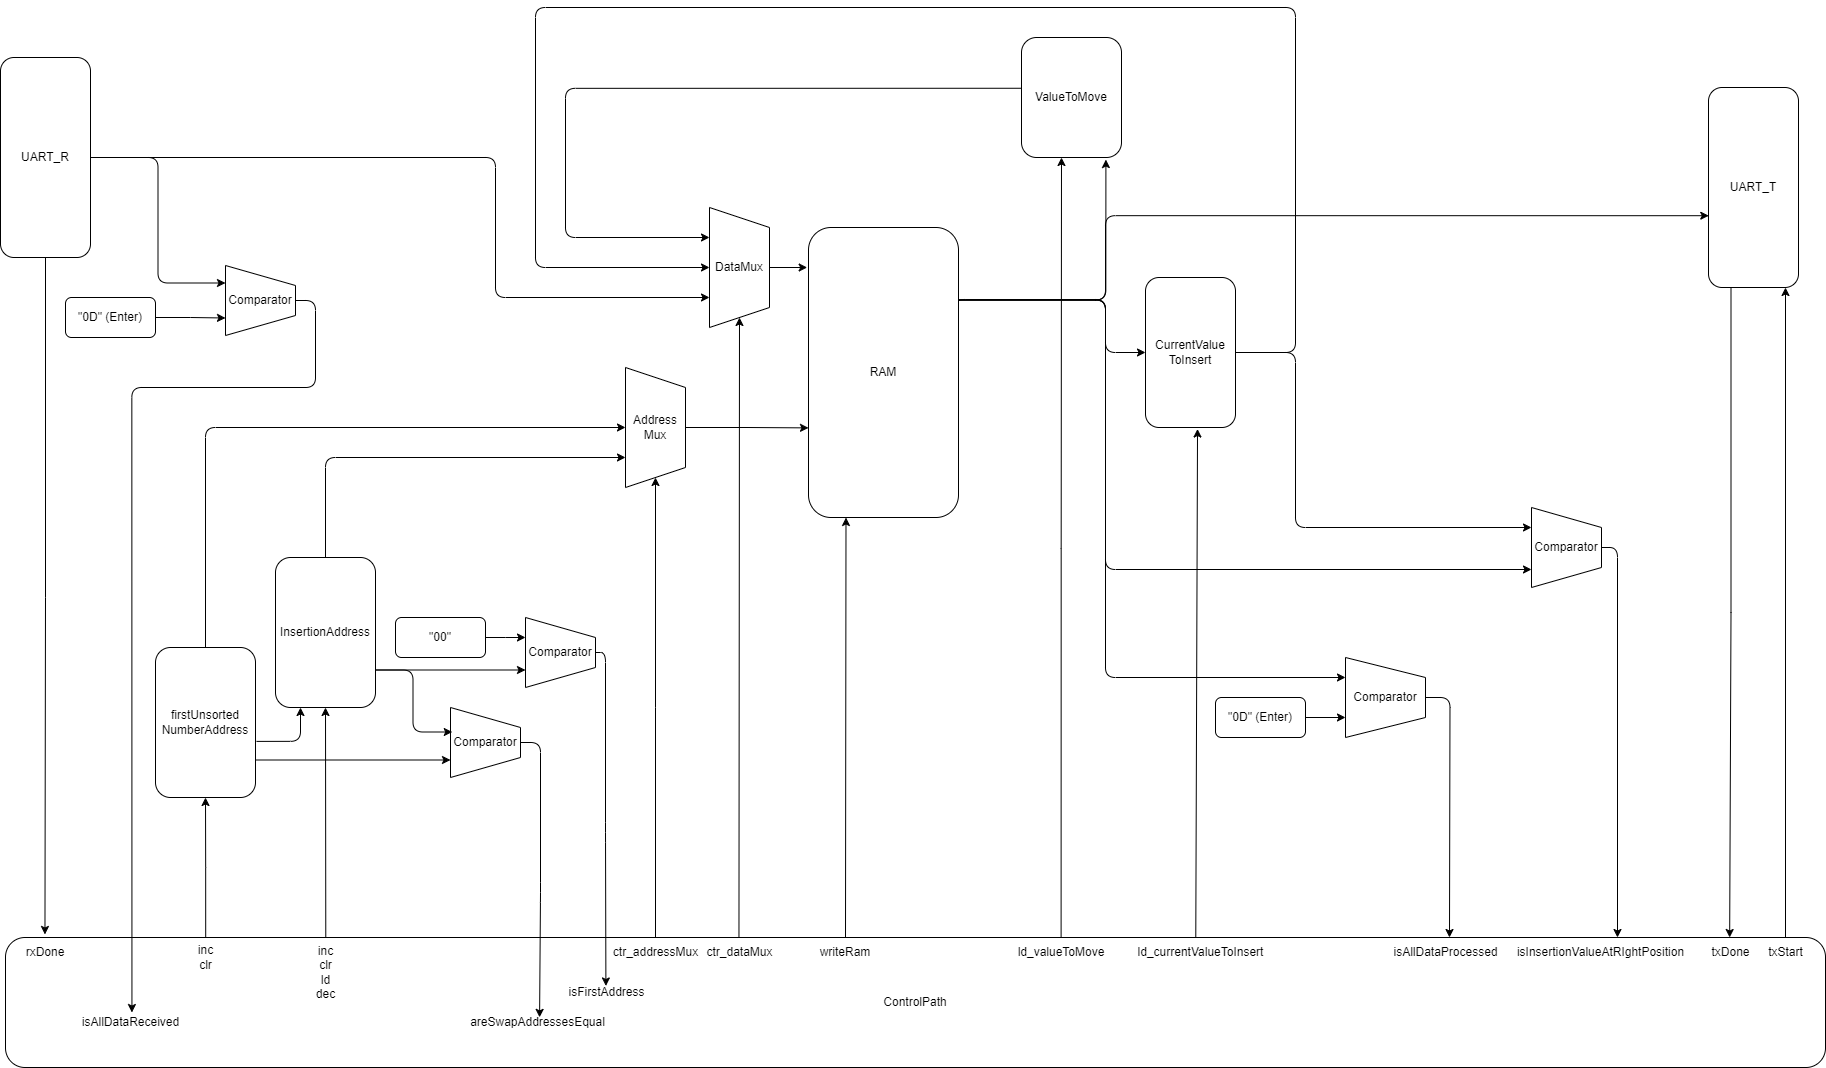
\includegraphics[width=1\linewidth]{Images/FSMDInsertionSort.png}
    \caption{FSMD diagram for Insertion Sort. The upper part represent the data path while the box below represents the control path.}
    \label{fig:fsmd}
\end{figure}
\begin{figure}
    \centering
    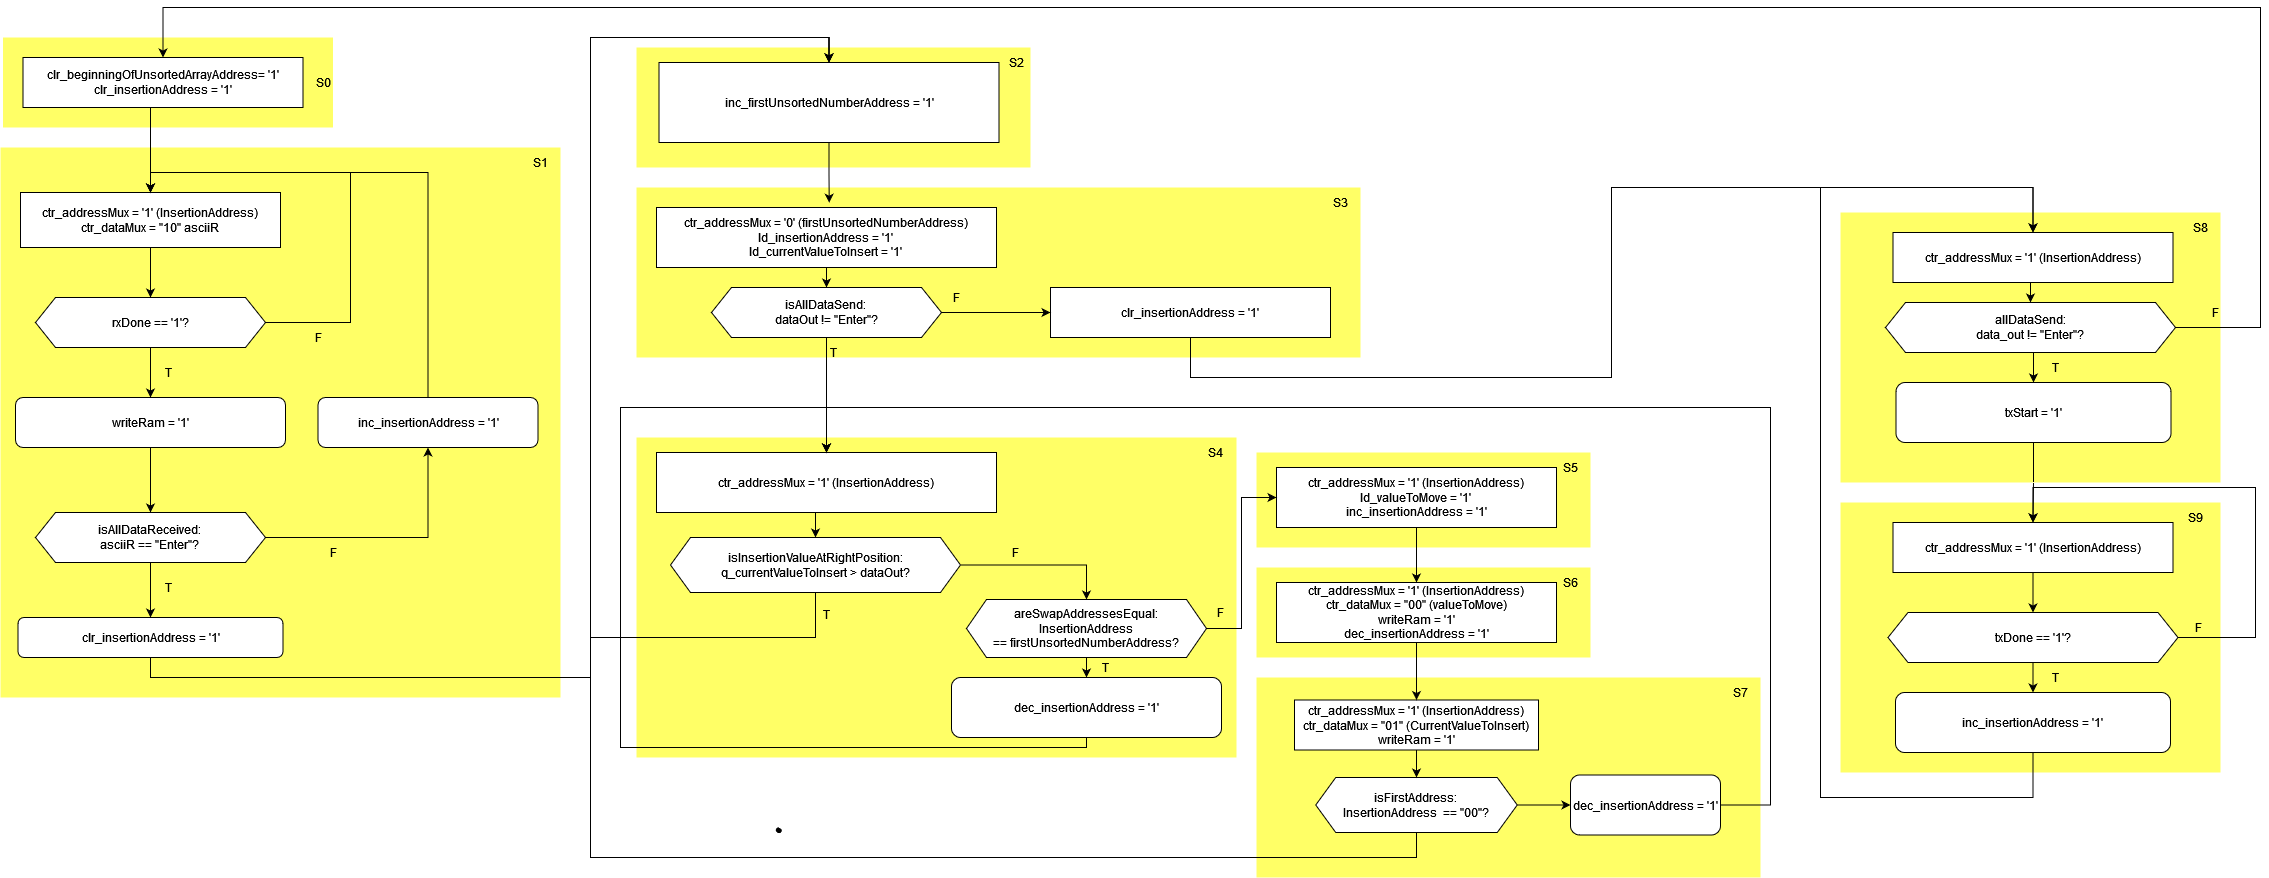
\includegraphics[width=1\linewidth]{Images/ASMDInsertionSort.png}
    \caption{ASMD diagram for Insertion Sort. The two states on the left represents the receiving of data. The six states in the middle represent the sorting algorithm itself and the two states on the right represent the output of the data via the \texttt{UART\_tx}.}
    \label{fig:asmd}
\end{figure}

\subsection{ASIP}
The second implementation was the ASIP, which we implemented using the logic of the ASMD chart. This allowed us to stay consistent with our design choices as well as keep a structred overview of the ASIP implementation. We went through the ASMD chart and converted the boxes into instructions. At first we converted the instructions into natural language before converting them in a second step into ASIP instructions. We used the one-cycle cpu design as a template for the ASIP design and modified it. This included adding additional components and control signals. The changes which we made, can be seen in TODO fix ref \ref{fig:asip} in light blue. The new components are an \texttt{uart\_rx}, \texttt{UART\_tx} for sending and receicing the serial data, a \texttt{comparator} for handling conditional statements and a \texttt{data\_mux} since we increased the amount of singals going into the data register. Both of the UART components have a start and a done signal. The \texttt{comparator} only has one output signal which goes trough the control path into the \texttt{pc\_mux}. The \texttt{data\_mux} only needs an input for controlling which data will be forwarded into the data register.\\
We used some of the registers only for specific values. For example, the \texttt{Reg[1]} was used to store the address of the first unsorted number in the array. These mappings can be found in the code above the instruction set.\\
Our instruction codes for the ASIP are devided into three logical sections. We go through these sections one by one and explain their idea as well as the reasoning for creating new instructions when necessary.\\
The first section - the first 8 instructions - handels the receiving of data and writing it into the \texttt{data memory}. Its starts of by resetting our two main pointers to addresses in the \texttt{RAM} that we use. Next we have a new custom instruction(\texttt{LOP\_UART\_DONE}). This instruction sends the \texttt{rx\_start} signal, writes the output from \texttt{UART\_rx} to the data registers and loops to itself until the \texttt{rx\_done} signal is received. The immediate value has to be 0 for this to work. This complex instruction was necessary since the \texttt{rx\_done} is only shown for one clock cycle and therefore needs to be checked every clock cycle. After receiving the data into a register, it is written into the data memory. Next we check if the data, which we just received, is an \textit{Enter}. This would stop the receiving of data and jump to the next section. This required an additional instruction code. Depending on the result of the comparisson, we either want to jump to a different section or continue with the next instruction. For this we created the comparisson component and connected it to the \texttt{pc\_mux}. Further we created three new instructions: Branch if Equal(\texttt{BEQ}), Branch if Not Equal(\texttt{BNE}), and Branch if Greater than(\texttt{BGT}). We only needed the first instruction for the first section but we implemented all of them at the same time since we knew that we would need the other instructions for later sections in the instruction code. Since the immediate value is used to specify the jump location, the comparisson is only possible between two registers.\\
The second section - the next 19 instructions - handels the sorting algorithm itself. We load the next value from our unsorted area in the array and compare it to an \textit{Enter}. This is to branch to the third section for the output since the \textit{Enter} indicates the end of the array. If the condition is not met, we know that we have a value which needs to be sorted. Next we try to find the position in which the unsorted value needs to be inserted. This is done by going from the back to the front until we find a value which is smaller or equal to the value which we want to insert. Therefore, we needed the new \texttt{BGT} command to do this comparisson. All values along the way are swapped until we find the correct place to insert the unsorted value. The swapping is handeled by instructions $0x12-0x16$. After swapping, we check check if we have reached the first address of the array. This would indicate that we can continue with the next unsorted value. Even though this section might seem to be complex, the logic itself is exactly the same as in the ASMD. Sometimes multiple commands are needed to reflect one box.\\
The last section - last 8 instructions - handels the sending of the data to the \texttt{UART\_tx}. Similar to the other sections, finding an \textit{Enter} value, will branch to the next - in this case first - section. Otherwise we send the next character via the serial connection until we find that \textit{Enter} value. This required two new instructions. One instruction \texttt{WR\_UART\_Start} is for starting the \texttt{UART\_tx} component with data from the \texttt{data memory}. The other instruction \texttt{LOP\_TX\_DONE} is a loop which is implemented quite similar to the loop in the first section. This time we loop until we receive the \texttt{tx\_done} signal.\\
The instruction memory had initially space for 32 instructions. We needed more than 32 instructions for our sorting algorithm. Therefore, we extended the instruction memory and all other signals which depend on it by one bit. \\
In the end we created six additional instructions, four additional components, 34 instructions in the instruction memory and we made a couple of changes to the exisiting components and code. The resulting behavior is exactly the same as it is for the FSMD. The code worked on the Basys3 board. The exact same behavior is achieved by relying heavily on the same ASMD diagram for both the ASIP and FSMD. Further information about the debugging, the implementation complexity and other aspects can be seen following subsections in the second part of the report. \\

\begin{figure}
    \centering
    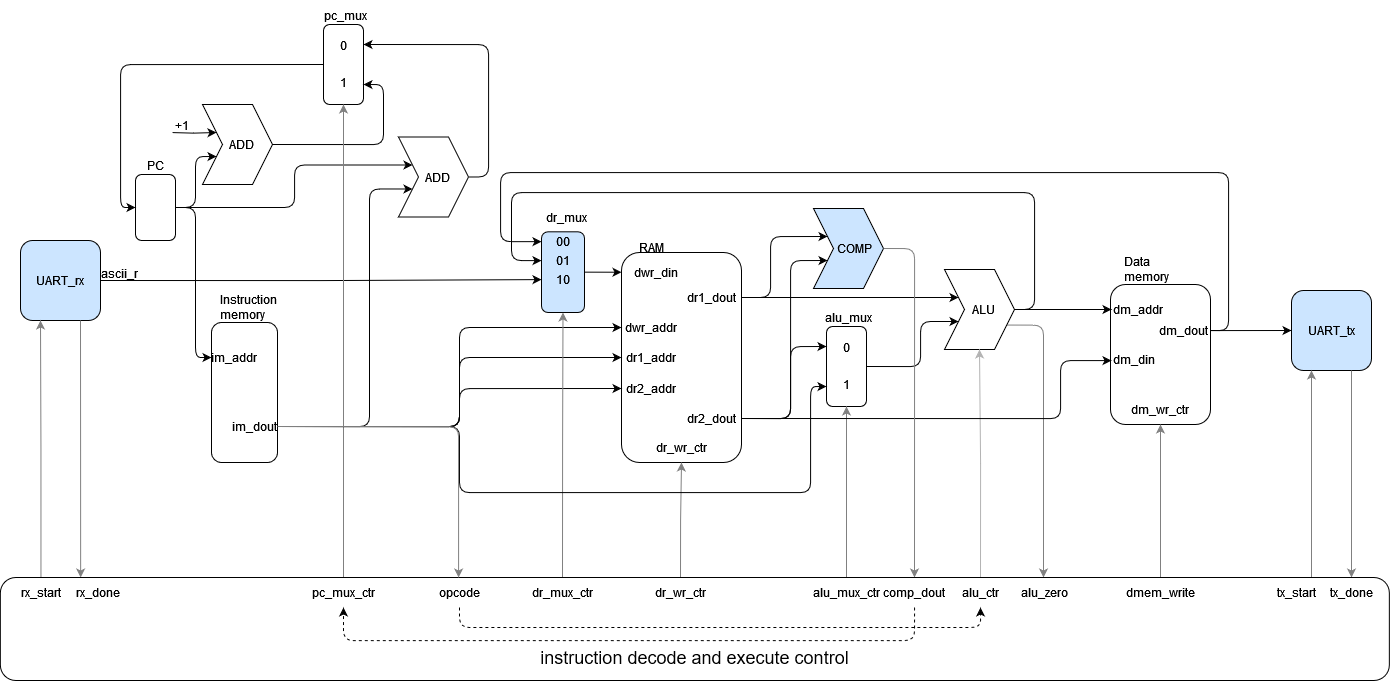
\includegraphics[width=1\linewidth]{Images/ASIP.png}
    \caption{ASIP diagram, based on the same ASIP diagram from the lecture week. The light blue components as well as their connections are new components to enable our Insertion Sort algorithm to be executed.}
    \label{fig:asip}
\end{figure}

\subsection{C coding in Vitis}
Next up, we definied the C program. We setup the project - as we have done it in the lecture week - based on the roadmap of Eric Peronnin. This was done to start on a working version which we could always go back to if and when encoutering errors. This proved to be a valuable resource since the debugger output was sometimes not very explicit. We started by removing the logic for the LEDs present in the code both in Vitis and afterwards in Vivado by removing the Blocks for the LEDs in the design. We then implemented a basic Insertion Sort algorithm in C from the code examples available in geeksforgeeks \cite{g4g}. Next we changed the input and output behavior. Utilizing \textit{print} statements for debugging, we managed to get the code working efficiently in a short time span. The majority of time spent on implementation and debugging mainly revolved around issues with pointers. Since no one in the group had any expertise in C, errors pertaining to pointers and similar issues were to be expected. We verified and tested that our final version of this implementation behaved on the Zybo board exactly the same as the FSMD and ASIP implementation did on the Basys3 board. Once we made sure the code behaved as expected we moved on to the next implementation.

\subsection{Create custom IP block}
Lastly, we implemented the IP block. We expected this to be very similar to the C porgram. As we have done it in the implementation before, we started based on a working version. To achieve this, we implemted the FIR Filter Project from the lecture week. \\
This implementation gave us the problems. The first issue we encountered was in the udpating of the components in Vitis. Vitis seem to have a cache which is not cleared automatically when updating components. So when we made changes in our High-Level Synthesis (HLS) component, created a new xsa file and updated the platform, we encountered the same behaviour as before. Only deleting the platform and application component in Vitis, fully seemed to clear any cached data. \\
Other issues were all based on the connection between our application component and our HLS/IP component in the platform component. As described we started of with the fir filter implementation. Since the fir filter implementation exchanges only single integer values, we wanted to modify it into sending arrays. An array cannot be set as an input for a function in C, so we used pointers to indicate the first value of the array. The values of the pointers were exchanged between these two components. Any further data was not copied. This meant that we could only exchange the first value of the array which is not sufficient for this task. Next, we tried a different angle to this issue by exchanging a struct between these two components. The issues with this idea were in the application component. We did not manage to find out how to use custom data types with the Xilinx library from AMD to send the information between the IP and software component. We also saw the option to share RAM between these two parts. However this seemed to be very complicated. We opted to switch back to the fir implementation and instead of using an array to exchange the data, we send the data one by one via the existing exchange of integer values. We managed to build a working version around that idea. After confirming that we have a working version, we refactored the code and finished that part of the implementation. \\
Most of the time for this implementation was spend on the issues that we had. The implementation of the sorting function and the implementation in the end were quite similar to the C-code implementation which we used as the starting point for this implementation. We estimate that we spend 75\% of our work in this implementation with dealing with the issues instead of coding and debugging. This can be atributed to both the lack of knowledge of the tools and libraries as well as a worse debugging experience which explain later in~\ref{sec:debugging} (TODO link to subsection). Due to these issues, we tried a lot of different approaches as well as using ChatGPT (TODO footnote). The solutions from ChatGPT did not prove to be valuable for us. Either it referred us to solution which worked in C but did not with the interface between the two components or it suggested solutions which were overly complicated.

\section{Comparison}
This section will evaluate the four implementations for different aspects. We chose aspects that should be considered when diciding for a specific implementation. Due to the small scale of the project, we do not aim to get specific numbers for each implementation. We rather aim to list the benefits and drawbacks which we learned in the scope of the project. We will conclude with a summary which implementation fits best for which requirement.

\subsection{Design and Implementation Complexity}
In this subsection we want to evaluate how complex it is to design and implement each approach. The FSMD and the ASMD are very close from the design complexity point of view since they rely heavily on each other. In section \ref{section:fsmd} the design process was already explained for these approaches. Even though the task was not easy we still managed to do it by contibutions of the whole team.\\
The implementation of the FSMD and the ASIP varied slightly from each other. The main difference here being the abstraction logic which is applied for the ASIP to enable the usage of instructions. In the FSMD we could use the states that where described in the ASMD directly. The statements in the ASMD are very close to the final code. While implementing we found out that we had some errors in our design, which could be fixed fast.\\ 
On the other side, the ASIP implementation needed more abstraction. We converted the states in multiple smaller opcodes, which were developped and then reused multiple times. We needed to figure out the right opcodes, define them and implement them correctly in our code. The abstraction was higher, the readability gets more difficult and thus errors could be overlooked more easily. Our main source was the lecture and the working code that we implemented while lecture week which helped a lot as a basis for the implementation. In the end the additional complexity did not contribute to more development which can be seen in \ref{sec:devcost}.\\
For the C implementation the designing was rather easy and straight forward. We used our knowledge of the sorting algorithm and the internet to come up with a first draft. For the implementation we used the draft and made small adjustments mainly to include a serial port for receiving and transmitting. We all have experience in coding and that can further add to the perceived ease of the implementation and complexity. \\
Starting the last implementation - the IP Block - we thought of an easy but yet clean design. We wanted to include the already finished C code in the example code of the FIR filter. To do so, we needed to send an whole array - with multiple cells - from the application component to the IP component in the platform component. We did not find a way to do this, reasons for this might be our missing experience in this topic and the lacking documentation on the internet. We came up with other design ideas such as trying to copy the array, creating a self-definied struct or to forward a pointer to the array. We implemented all of these ideas. However the various different debugging tools caused considerable issues which is described in more detail in \ref*{sec:debugging}. In our final design, we adapted the code closer to the exisiting FIR-Filter without any changes to the connection between these components. The complexity of the connection was too high for us to change it to something else outside of the example in the FIR-Filter. We were unaware of this additional complexity and it needs training in the libraries and tools to overcome this additional complexity.
%conclusion:
There were three implementations which had considerable design and implementation complexity and there was the C-code implementation without any considerable complexity. The complexity of the ASIP and the FSMD were quite similar. However, the ASIP had additional complexity due to the additional abstraction for the instruction codes. This complexity makes it harder to understand the algorithm form the code itself and further diagrams are needed since the code loses its ability to be descriptive. Therefore, when knowing exactly what algorithm has to be implemented, the FSMD implementation has an advantage. For both implementations, the complexity of the algorithm increases the complexity of the implementation. The IP block implementation has a fixed complexity which was in our case equal or even a bit higher compared to the direct implementations in hardware. This complexity came only from the connection between different components. More complex algorithms  will not increase the complexity of implementation in this case. Additional training will help to reduce complexity.\\
The implementation in pure software is the solution to avoid any complexity.\\

\subsection{Debugging and Verification Complexity} \label{sec:debugging}
After design and implementation we were debugging and vereifying our code. When deciding on an implementation one should consider the complexity of the debugging and verifying, since they vary greatly in our differnt approchaes. In both the FSMD and the ASIP, we used the simulation in Vivado. In both cases we had to customize the signals that we want to simulate. The difficulty with this debugging lies in finding the first unexpected or abnormal change. In both cases we used both our diagrams to go through the flow and compare our expected values to the simulated values until we found the outlier. This resulted in two or even three people doing the debugging. Since we worked as a team on this task, this did not present any resource issue. Nevertheless, this form of debugging felt slower and more complicated compared to debugging python code in a modern IDE in which you can mark the line of code, to which you want to jump. Although being a slow process, it still proved to be an effective tool to find any mistakes that we made. We managed to find all our mistakes with this form of debugging. One benefit of this debugging method is that you do not have to know where you want to debug. Since you get many singals at once, the abnormal behaving signal is very likely included. This reduces the amount of restarting the debugging procedure itselfs. \\
For the C-program we used print-statements for debugging. We viewed the output directly via the serial connection in putty. This form of debugging was quite familiar to all team members. It was intiutive and faster compared to the method above, since we did not have to search for the abnormal signal. However the print-statements have to be included in various places and also have to be deleted afterwards. The code is therefore changed for debugging. Despide this downside we managed to debug quite a bit faster than the first method. \\
Even though the IP block is written in C, the debugging experience is quite different and more complex than in the method before. Since there are seperated components, the complexity increases and there are more things which can work or not work and need therefore debugging. The building of the HLS component and afterwards the C-simulation could be debugged as normal C-code. The difficulties start at the RTL simulation. The RTL simulation could fail without giving good indications of the reasons for it. Further a working C-simulation is no indication for a working RTL simulation. This could be due to issues in transfering data, not sending data or running into a loop which was not cought in the C-simulation. As far as we could see, there is not even a debugging tool for the RTL simulation. Our solution was to uncomment sections of the code until we find the section which causes the issue. This is complex and prone to errors since the code logic is heavily effected by the debugging. When the RTL simulation worked, it produced a waveform file. However this waveform file was more complex and difficult to understand since there are many signals in the waveform file to represent the logic of the C code. However, the signals are auto generated and therefore have unintuitive names. We tried debugging with this but could not make any use of it. The next point of debugging is in the application component. At this point there are many possible areas in which the bug itself could be located. This means that we can print the values which we send and receive to the IP block but depending on the results, we cannot located the bug clearly. Due to the lack of knowledge of this interface between the components, we made many mistakes with the interface itself which were neither located in one or the other component and were therefore difficult to debug. \\
The different implementations result in various different debugging experiences and required skills for debugging. We spend the most time for debugging on the last implementation which was unexpected. The complexity of the interaction between the various different parts resulted in a complex debugging process. Further, the lack of tools for debugging this complex situation, resulted in a slow process. The third implementation was by far the fasted to debug. Both the first and the second implementation took some time to debug but it was still manageable and there was steady progress in the debugging. The last implementation was very difficult to debug and it was unpredictable how fast an error could be found. This should be taken into the cost consideration for the implementation.

\subsection{Flexibility, Reusability and Maintainability}
The flexibility, adaptability and reusability of the solutions varies a lot. Our first implementation is completely written in VHDL. The FSMD was just specificly designed for this sorting algortihm. There is nothing flexible in this implementation. If we want to change the sorting algorithm, we would have at least to redesign the full control flow. Depending on the sorting algorithm, we might need more additional components. Everthing must likely be renamed and restructured. At that point a new algorithm would effect anything in the code but the most basic components. Any other algorithm besides sorting algorithms would likely change the code completely. Anything which is already implemented in hardware has to be changed fully or is not reusable. \\
The ASIP implementation is a little bit more flexible. A change in sorting algorithms changes the control flow. However it depends on the sorting algorithm if anything else needs to be changed. Since the instruction set can be reused for anything, similar algorithms can also be run on the ASIP. Just the instruction memory needs to be exchanged. This enables small changes even after the hardware is created. However the complexity of implementing a change is rather high. It is not easy predictable what consequences a single new instruction can have on all other instructions. \\
The fourth implementation is more flexible than the first two implementation. The huge flexibility benefit comes the fact that is it not specified how the IP blocks are used. The IP blocks act as predefined algorithms which are likely to be used and optimised. What data and how the data flows into these algorithms, is not specified at the time of creating the hardware. Since there are many algorithms for different standards, this concept can be seen in many modern computers and chips. Standard algorithms for video encoding and deconding can be implemented directly into the hardware. Other algorithms for hashing or encryption/decryption of messages can also be implemented in hardware to increase the speed of opertaion. Any mistakes in the implementation of the IPs, can however still result in high costs and broken products if this is not detected before creating the hardware. \\
The third implementation is the most flexible implementation. In this implementation there is nothing specific about the hardware. The code can be deployed to any hardware which can run the C-code. Any mistakes in the code can be fixed by redeploying the code to the hardware. Any new algorithms can also be deployed, additional functionality can be added afterwards and maintaining it is possible as long as the hardware does not break. This makes it undoubtfully the most flexible implementation. However at this point we lose the benefits of implementing algorithms in hardware. \\
The solutions one, two and four offer different kinds of flexibility. Depending on the clarity of requirements and the maintainability it might not be possible to chose the first or second implementation. Therefore, implementing a few crucial algorithms as IP blocks, might be the middle ground which is chosen to ensure that there is still enough that can be changed after creating the hardware. If even that is not possible, the only solution that remains is writing non hardware specific code.

\subsection{Efficiency and Execution speed}
% should we count the cell usage for the FSMD, ASIP and IP block for this section?
The following paragraph will analyze the efficiency of the approaches from various perspectives including execution speed, power consumption, and resource utilization. Since we are using two different hardware bords we do not want to compare the values we get for the execution speed, power consuption and the resource utilization from the boards directly. Due to the different hardware the foundation for a direct comparision is not given. In the next section we will thus concentrate on the theory behind this efficiency of the implementations.\\
FSMD designs offer the highest level of efficiency in terms of execution speed and power consumption for fixed, predefined algorithms such as Insertion Sort. In FSMD, the algorithm is hardwired into a finite state machine with a dedicated data path, allowing for highly optimized data flow and minimal control overhead. As a result, a FSMD can execute the Insertion Sort algorithm in a very short time, often coming close to the theoretical minimum number of cycles for the given hardware. In terms of power efficiency, FSMD is typically superior due to its simple and optimized control logic, which minimizes switching activity and dynamic power consumption.\\
ASIP designs strike a balance between flexibility and efficiency. While ASIPs are not as efficient as FSMD in terms of execution speed and power consumption, they offer significant flexibility due to their programmability. The Insertion Sort algorithm can be efficiently implemented using a custom instruction set, which allows for hardware-level optimizations specific to sorting tasks. ASIPs can also leverage parallelism and pipelining techniques to enhance their efficiency, making them suitable for applications that require performance with the flexibility to handle a variety of tasks. The additional states which an ASIP has compared to an FSMD are the main difference in additional power consuption and reduced efficiency.\\
The C implementation of Insertion Sort, running on a general-purpose processor, offers the lowest efficiency among the compared approaches. Since general-purpose processors are not optimized for specific tasks like sorting, execution is slower, and power consumption is higher compared to specialized hardware implementations. The control flow of the Insertion Sort algorithm in C involves multiple levels of abstraction, which leads to additional overhead.\\
A custom IP block synthesized using HLS is designed to achieve high efficiency with less design effort compared to a FSMD. By describing the algorithm in a high-level language (such as C or C++), HLS tools automatically generate hardware that is optimized for the target algorithm, including Insertion Sort. This allows for more efficient use of resources while offering some flexibility through design-level changes. Custom IP blocks can take advantage of architectural optimizations such as pipelining, data-level parallelism, and reduced memory access, leading to improvements in execution speed and power consumption. This approach is ideal for applications that need efficient hardware but also require rapid development cycles. The exchange of data between the IP block and the code running on the processor generates overhead which decreases the efficiency and speed. This solution is not as efficient or fast as the direct hardware implementations.\\
The most efficient approach depends on the application context. For maximum performance and minimal power consumption, FSMD is ideal. ASIP and custom IP blocks offer a good trade-off between flexibility and efficiency. From these aspects the C implementation is worse compared to the others.\\

\subsection{Concurrency}
% In think this section has to be done again.
In this next section we want to compare our four implementations under the aspect of concurrency. This aspect refers to the ability of a system to execute multiple operations or tasks simultaneously.\\
While the FSMD may seem like it is limited in its concurrency capabilities, this view is only partly correct. In each state, the FSMD can utilize concurrency, as many operations can occur simultaneously within a single state. However, tasks that directly affect one another must be split into separate states, limiting simultaneous execution for dependent operations. Despite this, the FSMD is fundamentally designed for sequential control flow, where the progression through states follows a fixed order.\\
ASIP designs offers less concurrency compared to FSMD. The ASIP splits up the states which we have in the FSMD into even smaller states. Each instruction represents one state. All these intructions and therefore states are executed in sequence. The instructions itself can have multiple concurrent changes but due to the design this is expected to be less concurrency compared to the FSMD. It might be possible to execute multiple instructions at once. This would be however far more complex to ensure that the instructions do not depend on each other. This is outside of the project scope. \\
Custom IP blocks synthesized using High-Level Synthesis (HLS) can achieve high levels of concurrency. HLS tools translate high level code into an optimized hardware implementation. In our project this was done by Vitis. This automatic translation can be highly optimized for concurrency. This makes custom IP blocks highly efficient in terms of concurrency which can then be used to handle large amounts of data for efficient with a smaller execution time.\\
With the C code we implement a pure software solution. Concurrency is definied on a hardware level. Without using libraries, compilers and hardware that are specialized on optimizing software code to run efficiently on hardware, we do not have any concurrency in place for the C code.\\
%conclusion
To conclude, custom IP blocks, ASIP and FSMD all offer a high level of concurrency. They can all be designed towards concurrency but the designer must ensure the accuracy of the algorithm. C implementations do not have a nature of concurrency. There would be solutions to run algorithms on multiple CPU-Cores but this is complex and a topic which is outside of the project scope.\\

\subsection{Development Cost} \label{sec:devcost}
This section aims to quantify the amount of time that we spend on each implementation and thereby give an estimation how the cost of the different implementations can vary. All three of us worked on all implementations at the same time. To reduce the complexity, the time we spend on each implementation is only given as it would be for one person. If we for example spend one day working on an implementation, this would be noted as eight hours even though three people worked on it for eight hours which would result in the actual time of 24 hours. This is done since we want to focus on the relative development cost between the solutions instead of the actual development cost.\\
For the FSMD development, we spend around 23 hours. This includes the time for the diagram, code refactoring and debugging until the implementation worked. Even though we cannot quantify it exactly, we spend a significant amount of time on the initial design. We created both the FSMD and the ASMD diagrams first and this took around six to eight hours. The second day was mainly spent on implementation and it ended in first tests and debugging. The rest of the hours were spend on refactoring, smaller improvements and getting every edge case to work without any issues. This implementation had a steady progress throughout the whole time.\\
For the ASIP development, we spend around 20 hours. Since we used the ASMD diagram heavily for this, we did not have to develop any new logic. This contributed to the ASIP implementation taking less time than the FSMD implementation. This was unexpected to us. We thought the ASIP implementation would take around 10\%-30\% more time than the FSMD implementation. Instead it was the other way around. During the ASIP implementation, we spend around the first ten to twelve hours on creating the logic and changing the existing processor. The last six to eight hours were used for debugging and refactoring. It also helped that we already debugged the FSMD first. We were more trained on the debugging process and we had little to debug. \\
For the C-Code implementation it took us about seven and a half hours to do the full implementation and getting the code to run on the Zybo board. Most of the time for this implementation was spent on setting up Vitis and debugging issues with pointers. Since we took an implementation from a reputable source, we spend little to no time on the algorithm itself. We did not have a lot of experience with pointer handling thus we made some mistakes here.\\
For the C-Code implementation with the IP block, it took us around 21,5 hours to get a working version. We spend around four to six hours on the actual coding and rest of the time with debugging. Reasons for this were very long compiling times in Vitis and Vivado, our missing understanding of Vitis and the connection between the software and hardware component. We underestimated both the complexity of this task as well as the time that we are going to spend on this implementation. Our progress was far from linear. Six hours before finishing the implementation we still were unsure about the logic.The algorithms for receiving, sending and transferring between the different components were still unclear at that point. This uncertainty should not be underestimated. The lack of knowledge caused considerable delays in this implementation. \\
We had three implementations which roughly took the same amount of time and one implementation with around a third of the time. The short implementation was done purely in software while all other implementations had at least a hardware component. This shows that the development costs are considerably higher for hardware implementations compared to pure software projects. We expected to have a larger time difference in the implementation time between the different hardware implementations. The time consuming aspects for FSMD and ASIP were the complexity of the implementation while for the IP Block it was the developing software. Our project task was likely not complex enough to differentiate in fine detail between the implementation cost for the different hardware implementations.\\

\subsection{Production Cost}
In this next paragraph we want to evaluate production costs of each approach. We will focus mainly on the hardware production costs which will include the non-recurrent costs (NRC) and the per-unit costs. NRE costs refer to one-time expenses incurred during design and development, while per-unit costs account for expenses related to manufacturing each individual unit of the hardware or software. Since we only used the development boards which are not used in a final product the following paragraph contains mainly theory that is referred to our project.\\
The FSMD approach involves designing a specialized hardware circuit for the Insertion Sort algorithm. FSMD designs typically require substantial NRE costs because of the need for specialized hardware tailored specifically to the Insertion Sort algorithm. After design verification, the physical fabrication of FSMD on silicon chips involves high initial costs, particularly for smaller production volumes. The cost per unit decreases with large-scale production but remains high due to the dedicated hardware architecture. For general use cases, the initial design and fabrication costs present significant barriers.\\
ASIP is similar to the FSMD. It needs a specialized hardware for the implementation for our Insertion Sort algorithm. Just like the FSMD we expect high NRE costs and also high per-unit costs which will drop by increasing the production volume.\\
The C implementation of Insertion Sort runs on general-purpose processors with a standard instruction set architecture (ISA). It requires no specialized hardware. The cost structure for C implementations is radically different from hardware-based solutions like FSMD and ASIP. The NRE costs for C implementations are minimal, as they require no custom hardware design. Since C implementations run on off-the-shelf hardware, the per-unit production cost is negligible. 
While the C implementation offers the lowest production costs, it sacrifices performance and power efficiency compared to FSMD and ASIP. Therefore, it is best suited for general-purpose applications where cost is a primary concern and performance can be compromised.\\
A custom IP block is developed using High-Level Synthesis (HLS), where a high-level language like C or C++ is used to define the algorithm, and the design is synthesized into hardware. This approach provides the flexibility of software design with the performance benefits of hardware.The NRE costs for custom IP blocks using HLS are lower than those for FSMD because HLS allows for the automatic generation of hardware from high-level descriptions. This reduces the manual effort required in hardware design, cutting down verification time and labor costs. The per-unit production cost for custom IP blocks is similar to FSMD since the synthesized hardware still needs to be fabricated on silicon. However, the flexibility in design allows for optimization, potentially reducing chip area and power consumption, which can lower per-unit costs. The custom IP block approach strikes a balance between development effort and hardware efficiency. While the NRE costs are higher than for a pure software solution, they are lower than FSMD and ASIP.
%conclusion
The production costs of FSMD, ASIP, custom IP blocks using HLS, and C implementations of the Insertion Sort algorithm differ significantly. FSMD and the ASIP incurs the highest costs due to the custom hardware design and fabrication, making the FSDM suitable for specialized, high-performance applications. The ASIP offers more flexibility with approximately the same price class. Custom IP blocks using HLS provide an efficient trade-off between flexibility and hardware performance. The C implementation is the most cost-effective for general-purpose hardware, with minimal development and production costs but lower performance. 

\section{Conclusion}
We implemented an Insertion Sort Algorithm in four different ways. We learned a lot about each implementation during the process of designing, implementation and debugging. Each implementation has benefits in certain areas as well as drawbacks in other areas. It depends on the requirements to select the suitable solution and to use the benefits of the solution as an advantage. We want to conclude the report to highlight situations in which we would opt to use each of the implementations. \\
The FSMD is perfect for scenarios in which the complexity of the algorithm is limited. Concurrency is a feature that can be supported here and thus an efficient and elegant solution can be supported. Nevertheless, there should be a strong requirement for this efficiency which justifies the extra costs of implementing the algorithm in hardware. The scenario and the requirements should be stable and fully definable before the projects starts. Any major changes would increase the costs and force a complete restart of the implementation. \\
When the requirements are not fixed in place, the ASIP solution can tackle these drawbacks from the FSMD. There is a certain amount of flexibility in the hardware implementation due to the additional abstraction. This comes at the cost of efficiency and execution speed. The ASIP also increases the complexity slightly compared to the FSMD. \\
When the efficiency of hardware is needed as well as the flexibility of a software implementation, the creation of custom IP blocks is the way to go. This solution aims to get the benefits of both hardware and software implementations. However, this results in a complex software environment for the implementation. It requires additional training and has the most uncertainty of the implementations so far. Furthermore, the solution is not quite as efficient and can not match the speed of a pure hardware implementation.\\
The software implementation in C has its benefits on the cost and flexibility side. Neither of those can be matched by any other solution. The implementation is likely to happen faster and the code does not require any specific hardware to run. The complexity is quite low compared to the other implementations. The additional abstraction with a high level programming language make it more readable and understandable compared to VHDL. But features like concurrency on hardware-level cannot be supported.\\

\section*{Acknowledgment}

We confirm that there was no significant difference in the contribution to the work.

\printbibliography

\begin{appendices}
\section{Use of AI}
used for write production cost section promt: Please write a one page scientific latex report as a professor of Computer science. The topic is the cost comparison between the production of FSMD, ASIP and a C implementation of a Insertion Sort algorithm. Please use a scientific writing style and include all sources that were used. Remember to write your report in latex code.
\end{appendices}

\end{document}
